\documentclass[../main-v1.tex]{subfiles}
\begin{document}
\chapter{Resource Needs Summary\hideme{coll-org.tex}}
\label{ch:resource}

\section{Hardware Resources}
Chapter~\ref{ch:est} describes the projected compute and storage needs through 2040, many of which are being met through collaboration contributions. Chapter~\ref{ch:netw} describes networking. 



\section{%Personnel Needs
Human Resources} %anne: seems to be the more current term in use
Building and managing a project of this complexity also requires a large number of %personnel
dedicated people.  Figure~\ref{fig:resources} shows a timeline for estimated human resource needs.   Efforts are currently spread across a large number of highly expert people working part-time on DUNE computing, aside from the five dedicated \dword{doe}-funded postdocs.  We anticipate that these early-career people will move into leadership roles in computing in the future.  Although the current FTE %are 
number is close to %the number 
what is needed, there is some mismatch in skill sets. In particular, we anticipate needing several person-years of effort on framework development, which is not available in the current mix of personnel.

%These roles do not include the large number of people at multiple sites who support generic activites such as storage and grid activities.  The roles listed are people working on \dword{dune} specific projects. 
The listed roles are limited to people working on DUNE-specific projects and do not include the large number of people at multiple sites who support generic activities in areas such as storage and grid.  


\subsection{Technical Roles}
\label{subsec:coll-org:Tech}

Technical roles require substantial computing expertise.  They appear as the darker areas in Figure~\ref{fig:resources}, adding up to approximately: 

\begin{description}


% FTE	2022
% Database administration	0.5
% Database devel. and ops	4
% Data management devel. 	3
% Workload devel. 	1
% Monitoring devel. 	1
% Code management devel. 	1
% Framework devel. 	1
% Analysis devel. 	1
% Data management ops 	2
% Workload ops	2
% Monitoring ops	0.5
% Code management ops	1
% User Support and Documentation	2

\item {Distributed Data Management Development -- 2.0 FTE}

This role includes oversight of all software engineering and development activities for packages needed to operate distributed storage resources. The role requires a good understanding of the distributed computing infrastructure used by DUNE as well as the DUNE computing model.

\item {Distributed Computing Development -  2.0 FTE}

This role includes all software engineering and development activities for packages needed to operate  distributed compute resources. The role requires a good understanding of the distributed computing infrastructure used by DUNE as well as the DUNE computing model.

\item {Monitoring Development -- 1.0 FTE}

This role includes oversight of all software engineering and development activities for packages needed to monitor distributed disk and compute resources. The role requires a good understanding of the distributed computing infrastructure used by DUNE as well as the DUNE computing model.

\item {Database Design, Development and Management -- 4.5 FTE}

This role includes designing, developing, maintaining, and scaling databases for  
tasks within DUNE. Considerable effort is needed to interface with the large number of physics, calibration, data acquisition, and hardware tasks. People are needed with expertise in databases, data acquisition, and project management.  Database administration effort for direct database interventions and operations are included here as they require specialized skills. The strategy is that the majority of the development Database effort will evolve into operations roles (see section \ref{subsec:coll-org:Ops}) as a way of retaining expertise and allowing future upgrades of the database infrastructure\footnote{It is noted that many experiments have reported difficulties in retaining database expertise which can result in greatly increased risk over time as technologies evolve.}.

\item {Code Management Development -- 1.0 FTE}

The code managers provide infrastructure to support applications for  data processing, simulation, and analysis, and also to coordinate activities in the areas of development, release preparation, and %properly
deployment of software package releases needed by DUNE. They organize the overall setup of software packages needed for releases.

The application managers need to keep up with evolution in operating systems, build systems, and compilers, so this role has a significant development component.

\item{Simulation, reconstruction and analysis frameworks -- 3 FTE}

This role requires substantial expertise in the design and deployment of sophisticated frameworks for HEP algorithmic workflows. 


\subsection{Operational  Roles}
\label{subsec:coll-org:Ops}
In addition to the development activities listed above, there are management and operations activities that require management and supervision of collaborators in operations tasks.   These roles are more fluid, based on the status of the experiment and do not always need trained computing personnel but can be filled by collaborators after some training. 
% \item {Central Services Manager and Operators - 1.5 FTE}

% The site manager and operators are responsible for the central infrastructure and services of the \dword{dune} distributed computing infrastructure. This includes coordination with the host laboratory for services provided to \dword{dune}. 

\item {Distributed Production Management -- 0.5 FTE}

Distributed production managers are responsible for the setup, launch, monitoring, and %finishing 
completion of processing campaigns executed on distributed computing resources for the experiment. %Production management is necessary for 
These include data processing, \dword{mc} simulation, and working group productions. 


\item {Distributed Data Manager -- 0.5 FTE}

The distributed data manager is responsible for operational interactions with distributed computing disk and tape resources. The role includes but is not limited to helping to establish new storage areas, and data replication, deletion, and movement. 

\item {Distributed Workload Manager -- 0.5 FTE}

The distributed workload manager is responsible for operational interactions with distributed computing resources. The role includes activities such as helping to establish grid and cloud sites. 


\item {Computing Shift Leaders -- 1. FTE}

The shift leader is %mainly 
responsible for the experiment's distributed computing operations for %a 
week-long periods that run Monday through Sunday.  %one person covers shifts 
%starting on a Monday to the following Sunday.  
Shift leaders chair regular operations meetings during their week and attend general DUNE operations meetings as appropriate. %1.4 FTE as it also includes week-ends.

\item {Distributed Computing Resource Contacts -- 0.5 FTE}

Distributed computing resource contacts are the primary contacts for the DUNE distributed computing operations team and for the operators of large (Tier-1) sites and regional federations. They interact directly with the computing shift leaders at operations meetings. 


\item {Code Management Operations -- 1.0 FTE}

In addition to development associated with changes in systems, code librarians and application managers must continually prepare releases and %properly
deploy  software packages needed by DUNE.  

\item {User Support -- 2.0 FTE}

User support (software infrastructure, applications, and distributed computing) underpins all user activities of the DUNE computing project. 
User support %also includes 
personnel %who 
respond to questions from users on mailing lists, Slack-style chat systems, and/or ticketing systems, %as well as documented 
and are responsible for documenting solutions in knowledge bases, FAQs and wikis. %\fixme{but not the FAQ?}

\item {Resource Board Chair -- 0.1 FTE}

This role is responsible for chairing quarterly meetings of the Computing Resource Board, which includes representatives from the %national \dword{dune} collaborations, 
various national funding agencies that support DUNE, to discuss %the level of 
funding for and delivery of the computing resources required for successful processing and exploitation of DUNE data. %0.1 FTE

\item {Computing Coordination - 2.0 FTE}

Coordinators oversee management of the computing project. 
\end{description}



\begin{dunefigure}
[Development personnel needs]
{fig:resources}
{Estimated computing infrastructure personnel needs through 2030.  The dark colors show development areas where experts are needed while the lighter colors show operations tasks where non-experts can contribute. The dashed line shows the estimated effort formally allocated to the project including additional effort from 2022-2024 from the three-year DOE grant and enhanced UK project funding.}
{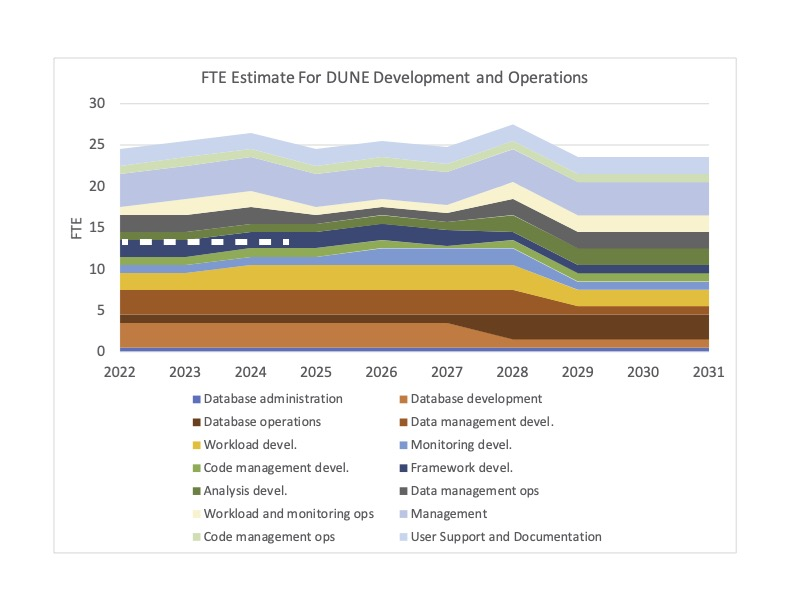
\includegraphics[width=0.9 \textwidth]{graphics/Resources/FTENeeds-2022-03.jpg}}
\end{dunefigure}
%\fixme{HMS - Need to restore the dashed line}

%\section{Summary}
%Kirby done. \fixme{this short section/blurb is unnecessary (anne)}
%This document has described most aspects of \dword{dune} offline computing. Our computing model relies on significant contributions across the collaboration.  

%\section{Computing Contributions Board}

%\hideme{Remove this chapter}
%%%%%%%%%%%%%%%%%%%%%%%%%%%%%%%
%\section{xyz}
%\label{sec:org:xyz}  %% fix label according to section
\end{document}
